\section{Importing a MySQL Database}
\label{sec:mysql_import}

After opening a database, import functions are available by clicking the 'Import' button:

\begin{figure}[H]
  \center
    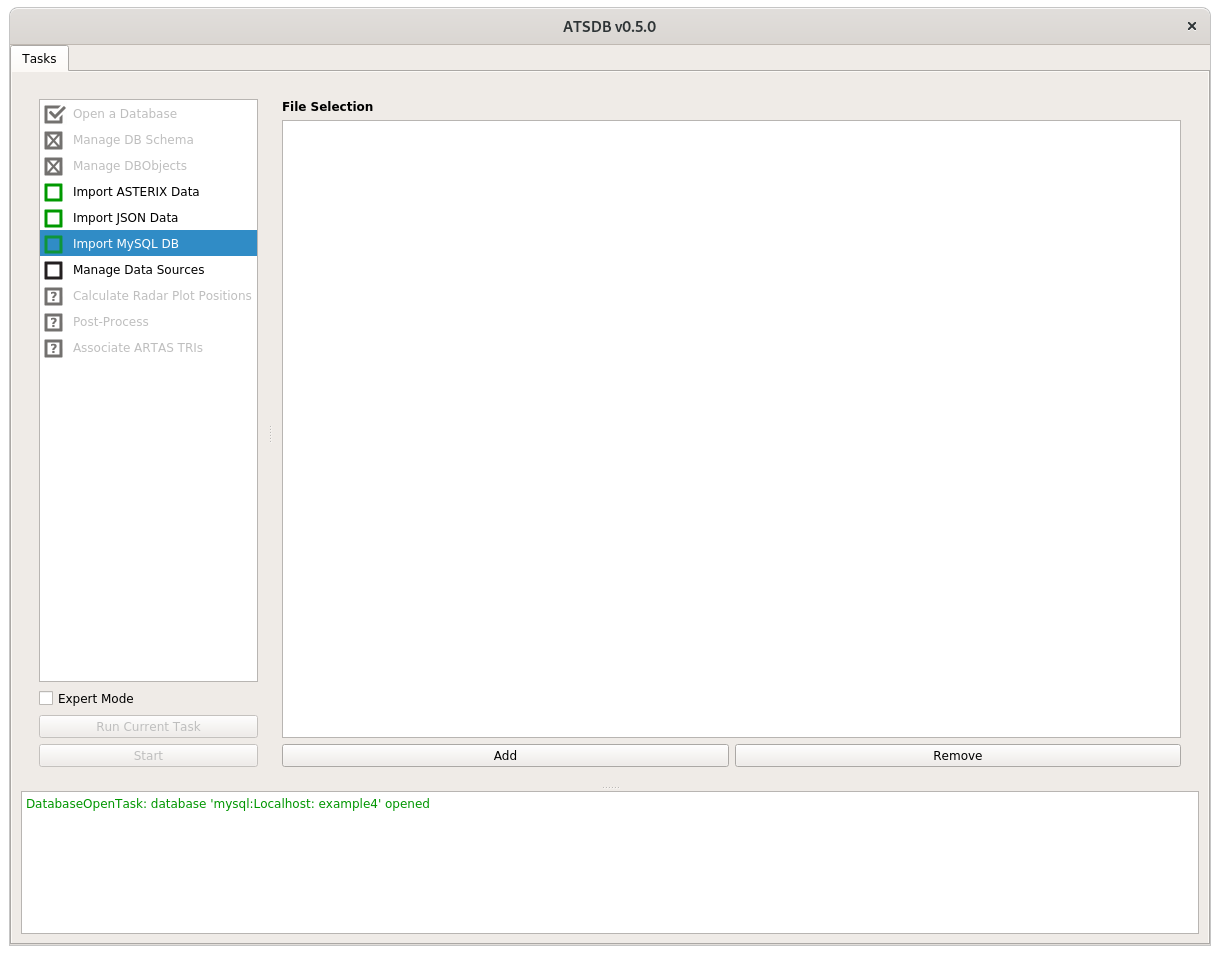
\includegraphics[width=9cm,frame]{../screenshots/database_import.png}
  \caption{Importing a MySQL database}
\end{figure}

\subsection{Importing a MySQL Text File}

A previously exported MySQL database can be read from a text file and written into the current database. After selecting this option, a file open dialog is shown which allows selection of '*.sql' files. Please note the following points:

\begin{itemize}  
\item The text file must contain valid MySQL statements
\item MySQL functions/views are not imported, only data which can be inspected
\item If more than 3 errors occur during the import process, it is aborted
\item If the import process was aborted, the current database might contain already imported parts which are not deleted automatically
\end{itemize}

\subsection{Importing a MySQL Text Archive File}

A previously exported MySQL database can be read from a text archive file and written into the current database. After selecting this option, a file open dialog is shown which allows selection of '*.tar.gz *.gz *.tar *.zip *.tgz *.rar' files. Please note the following points:

\begin{itemize}  
\item This function does \textbf{not} work to import an Verif-exported \textit{evaluation tgz}, but imports an \textit{SQL archive} from inside such an evaluation tgz
\item The text archive file must follow the same points as in the \textbf{Importing a MySQL Text File} section.
\item All files within the archive are read and imported into the database
\item If more than 3 errors occur during the import process, it is aborted
\item If the import process was aborted, the current database might contain already imported parts which are not deleted automatically
\end{itemize}

\subsection{Importing a SASS-C Evaluation Export}

The following steps must be taken:

\begin{itemize}  
\item An export from a SASS-C evaluation must exist, e.g. 'example.tgz'
\item Using your favorite archive manager, extract the file 'tgz-tmp/<JOB\_NAME>/exported.sql.gz'
\item After successfully connecting to a server, create a new database, e.g. '<job\_name>', and open it
\item Click on the 'Import' button and select 'Import MySQL Text Archive File'
\item Select the previously extracted 'exported.sql.gz'
\end{itemize} 
